\chapter{Réalisation du projet}

\section{Préparer les données}
\section{Explorer les données}
\subsection{Premières expérimentations}
Les premières explorations des données formatées sur 5 mois (issues du fichier PV.csv) nous ont permis d'identifier les élements suivants :

\begin{itemize}
\item Les données de production sont fournies par jour entre 6h50 du matin et 17h.
\item Il existe des jours avec des données manquantes
\item Les onduleurs exhibent des profils et des comportements parfois assez différents entre eux. Cette piste sera plus approfondie par la suite.
\item On remarque la très forte corrélation entre l'irradiance et la production électrique des panneaux photo-voltaïques. L'irradiance suit une courbe en cloche avec un pic autour des 13h-14h. La production électrique stagne autour des 900 $Wm^2$ mettant en avant les limites de production des panneaux solaires. 


\begin{figure}[!ht]
\begin{center}
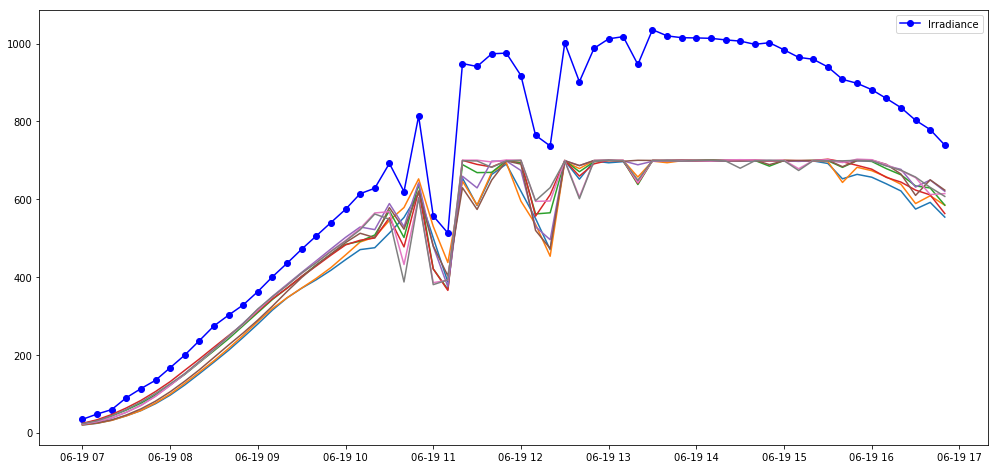
\includegraphics[scale=0.3]{rapport/images/Ch6_Irradiance-Prod.png}
\end{center}
\caption{L'irradiance et la production des 8 onduleurs pour le 19 juin 2018}
\end{figure}
\FloatBarrier
\paragraph{}
\item On peut observer que le modèle prédictif basé sur les données météorologiques est moins précis que son homologue. Il ne tient pas compte du phénomène de plateau contrairement au modèle basé sur les valeurs voisines dont les prédictions sont très précises :

\begin{figure}[h!]
\begin{center}
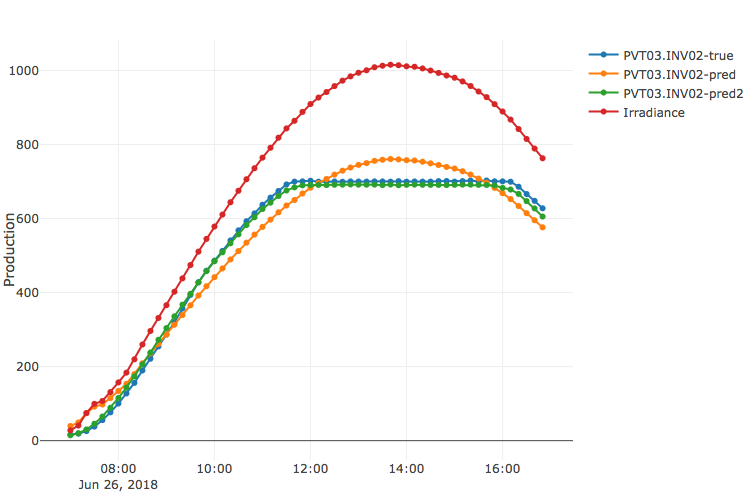
\includegraphics[scale=0.4]{rapport/images/Ch6_26juin.png}
\end{center}
\caption{L'irradiance et la production pour le 26 juin 2018, onduleur PVT03.INV02}
\end{figure}
\FloatBarrier
\item On constate que certaines journées sont très "bruitées" au niveau de l'irradiance, correspondant vraisemblablement à des journées nuageuses ou avec de la pluie, ce que nous tâcherons de mieux comprendre grâce à la décomposition du signal.
\end{itemize}

\section{Décomposer le signal}
\section{Identifier les signatures particulières}
\section{Rechercher les similarités}
\section{Répertorier les anomalies}
\section{Valider la classification}
